\RequirePackage{lineno}
\documentclass[conference]{IEEEtran}
%\documentclass[draft, onecolumn]{IEEEtran}
% correct bad hyphenation here
\hyphenation{op-tical net-works semi-conduc-tor}

% =============+s\\==================================================
%\usepackage{subfigure, graphicx, booktabs}
%\usepackage{algpseudocode, algorithmicx, algorithm}
\usepackage{amsmath, amsthm, listings, booktabs}

%Code environment
\newcommand{\code}[1]{{\tt#1}}
\newcommand\inputsrc[1]{{\tt \lstinputlisting[]{source/#1} }}
\long\def\comment#1{}

\def\ssp{\def\baselinestretch{0.99}\large\normalsize}

%\addtolength{\columnsep}{-3mm}

% setup listing parameters
%\lstloadlanguages{c++,c}
\lstset{language=c++,basicstyle=\scriptsize}
\lstset{numbers=left,numberstyle=\tiny,stepnumber=1}
%%\lstset{labelstep=1}
%\lstset{stepnumber=1}
%\lstset{stringspaces=false}
\lstset{stringstyle=\tt}
%\lstset{singlecomment={/*}{*/}}
%\lstset{commentline=/*}
\lstset{commentstyle=\it}
\lstset{morekeywords={new, exit, entry, Function, At, pid_t, u_int,
u_int32_t, FILE}} 
%%\lstset{indent=6mm}
\lstset{xleftmargin=4mm}

% *** GRAPHICS RELATED PACKAGES ***
%
\ifCLASSINFOpdf
   \usepackage[pdftex]{graphicx}
  % declare the path(s) where your graphic files are
   \graphicspath{{../pdf/}{../jpeg/}}
  % and their extensions so you won't have to specify these with
  % every instance of \includegraphics
   \DeclareGraphicsExtensions{.pdf,.jpeg,.png}
   \DeclareGraphicsRule{*}{mps}{*}{}
\else
  % or other class option (dvipsone, dvipdf, if not using dvips). graphicx
  % will default to the driver specified in the system graphics.cfg if no
  % driver is specified.
   \usepackage[dvips]{graphicx}
  % declare the path(s) where your graphic files are
   \graphicspath{{./}}
  % and their extensions so you won't have to specify these with
  % every instance of \includegraphics
   \DeclareGraphicsExtensions{.png, .pdf, .eps}
\fi

% ===============================================================
\newtheorem{theorem}{Theorem}[section]
\newtheorem{conjecture}[theorem]{Conjecture}
\newtheorem{corollary}[theorem]{Corollary}
\newtheorem{proposition}[theorem]{Proposition}
\newtheorem{lemma}[theorem]{Lemma}
%\newdef{definition}[theorem]{Definition}
%\newdef{remark}[theorem]{Remark}


\begin{document}
\title{A Template Metaprogramming Approach to Support Parallel
  Programs for Multicores}


% author names and affiliations
% use a multiple column layout for up to three different
% affiliations
\author{
\IEEEauthorblockN{Xin Liu, Minyi Guo, Daqiang Zhang, Jingyu Zhou, Yao Shen}
\IEEEauthorblockA{Department of Computer Science\\
Shanghai Jiao Tong University\\
No. 800, Dongchuan Road, Shanghai, P.R.China\\
navyliu@sjtu.edu.cn}
}
%\{guo-my\}@cs.sjtu.edu.cn,
%\{zhangdq\}@sjtu.edu.cn, \{zhou-jy, shen\_yao\}@cs.sjtu.edu.cn
% make the title area
\maketitle


\begin{abstract}
In advent of multicore era, plain C/C++ programming languages can not
fully reflect computer architectures. Source-to-source
transformations help tailor programs close to contemporary
hardwares. In this paper, we propose a template metaprogramming
approach to support parallel programs, which performs
source-to-source transformations for specific
multicores. Our approach is purely library-based, which represents parallel patterns and
executions as template classes. We implement a prototyped
template library -- Libvina, to demonstrate the idea. It enables
programmers to exploit new architectural
features and apply new parallel patterns by extending the library. 
Finally, we evaluate our template library on
commodity CPU and GPU platforms by a variety of typical procedures
in multimedia and scientific fields. In experiments, we show that our
approach is flexible to support multiple parallel models and capable
of transforming sequential codes to parallel equivalences according to
specific multicore architectures. 
%Moreover, the cost of programmability using our
%approach to adapt to more than one multicore is manageable.
\end{abstract}

% For peerreview papers, this IEEEtran command inserts a page break and
% creates the second title. It will be ignored for other modes.
\IEEEpeerreviewmaketitle


%\section{Related work}\label{sec:related}
%\begin{figure}
%  % Requires \usepackage{graphicx}
%  \centering
%  \includegraphics[width=0.8\linewidth]{../fig/motivation}
%  \caption{CFSF Motivation}\label{fig:motivation}
%  \label{fig:algorithm}
%\end{figure}
\section{Introduction}\label{sec:Intro}
%multicore problem
Modern computer architectures rely on parallelism and memory
hierarchy to improve performance. Both duplicated processors and
elaborated storage-on-chip require programmers to be aware of underlying
machines when they write programs. Even worse,
multicore technologies have brought many architectural features for
different implementations. Thus, it is challenging to develop
efficient applications which can take advantage of various multicores.

%need new programming model
In essence, it is because plain C/C++ programming languages
can not reflect contemporary architectures~\cite{cml}. Traditionally, programmers
describe algorithms in sequential logics, and then resort to  compiler
and hardware optimization to deliver modest performance relative to
their machines. In multicore era, this classic programming model gains
little. It is desirable to develop alternatives to utilize horsepower
of multicores while hiding architectural features.

% to aggresssive is not feasible
Although researches on revolutionary programming models have obtained
fruitful achievements, they are limited in specific
domains~\cite{gmapreduce, erlang, haskell}.
One critical issue hinders them from applying in general programming
field is that one programming model can only
benefit a small group of users. It is still unclear what
general purpose programming model is. Besides, the cost hardware usually weights
a small part in a computer system relative to software and
personnel. The ratio lowers with time. Therefore, vendors are
reluctant to adopt fundamental changes of software stacks for
multicore evolvement.

%Second, the cost of hardware in large systems
%is relative low than software and personnels. The ratio lowers along time
%pass. It is risky to drop up existing efforts and build software from
%scratch using new programming models.

An acceptable tradeoff is to extend traditional programming
languages to utilize effective parallel patterns. Appearently, the advantage of
this approach is that it can exploit multicores progressively. Thus the
knowledges and
experiences of traditional programmers are still useful, and investment
of legacy software is saved. In industry, OpenMP~\cite{openmp}  and
TBB~\cite{tbb} are successful cases. OpenMP provides parallel
programming API in the form of compiler directives. TBB is a C++ library, consisting of concurrent containers and
iterators. CUDA~\cite{cuda} extends C programming languate to describe
groups of threads for GPU. The limitation of preceded approaches are
platform or vendor dependent. In academia,
Sequoia~\cite{sequoia} attempts to programming for memory hierarchy. It
achieves parallelization by divide a task into subtasks hierarchically and then map
subtasks on nodes of machines. Merge~\cite{merge} implements
map/reduce programming model for heterogeneous
multicores. Streamit~\cite{ThiesKA02} compiler supports stream/kernel
model for streaming computation. Its run-time schedules kernels for specific architectures. The shortcoming of academical approaches is that each one
is capable of one type of parallel patterns.  In a word, existing solutions
lack uniform method to express multiple parallel patterns
across various multicores.

%FIXME: move to related works
%It(merge) relieson hierarchical division of task and predicate-based
%dispatch system to assign subtasks on matched multicore target at
%runtime. OpenMP and TBB are for shared memory system
%system such as SMP, while CUDA is property programming
%model for specific GPU architectures.

Observably, except TBB is a pure library-based solution, aforementioned
approaches need compilers to facilite their programming models. It is
the ad-hoc approaches embedded into compilers restrict flexibility and
extensibility. Therefore, we propose a template-based programming model to
support parallel programs for multicores. We exploit C++
metaprogramming techniques to perform source-to-source transformation
in the unit of functions. We use \emph{tasks} to abstract
computation-intensive and side-effect free functions, which are candidates for transformations. We extend the meaning of template
specialization~\cite{tcpl}. Our approach specializes a task for target's
architectures.  Through applying template classes, a task is
transformed into many subtasks according to different parallel
patterns, and then subtasks are executed in the form of threads.
Template classes are implemented for different multicore
architectures. As a result, porting software from one platform to another only
needs to adjust template parameters or change implementations of
template classes. The difference between TBB and our approach is that
we utilize C++ template metaprogramming, so the transformations complete
at compile time. 

%pros and cons
Our approach is flexible and extensible. Both parallel patterns and
execution models are provided as template classes, thus programmers can
parallelize tasks using more than one way. In addition, template
classes are organized as template library. It is
possible to exploit architectural
features and new parallelization strategies by extending library. We
explore language features limited in ISO
standard C++~\cite{c++98, c++03, c++0x}, so it is applicable for
platforms with standard-compilant compilers. Most 
platform-independent template classes can be reused. The limitation of
template-based approach is that using template metaprogramming, only compile-time
information is available. That includes static constant values,
constant expression and type information in C++. Therefore, our
approach is not a general solution and orients for programs with rich
static information. Fortunately, it is not uncommon that this
restriction is satisfied in the fields like embedded applications and
scientific computation. Because the runtime of those programs with fixed
parameters are significantly longer than compile time even the time to
write programs, it will pay off if can resolve transformations at
compile time. Besides, it is possible to utilize external
tuning framework~\cite{tuningfrm} to adjust parameters of static programs.

In summary, we proposed a template-based programming model, which 
tailors programs to multicores. Programers apply template classes to
transform functions into the parallel equivalences on source-level,
and then map them on specific multicores to run simultaneously.

%organization structure
The remaining parts of this paper are structured as follows.
Section~\ref{sec:model} presents our programming model. Section~\ref{sec:lib} introduces libvina
-- a prototype library to facilitate template-based programming model.
Section~\ref{sec:adaption} is how programers adapt their source codes to libvina. Section~\ref{sec:details} gives details of
implemetation of our library. Section~\ref{sec:eval}
evaluates performance on both CPU and GPU using our approach.
Section~\ref{sec:related} summarizes related work to support parallel programs
for multicores. Section~\ref{sec:con} is disscussion and future work.


%\section{Background}\label{sec:background}
\begin{figure*}
  % Requires \usepackage{graphicx}
  \centering
  \includegraphics[width=0.731\textwidth]{../fig/algorithm}
  \vspace{-2ex}\caption{Deriving CFSF from traditional CF approaches}\label{fig:cfsf}
  \label{fig:algorithm}
  \vspace{-2ex}
\end{figure*}

Recommender systems aim at predicting the rating of active item $i_a$
made by active user $u_b$ from user profiles. These profiles are
represented as a $Q \times P$ item-user matrix $X$, where $Q$ and $P$
are the sizes of $X$. In this section, we introduce notations for CF.
Let
\begin{itemize}
  \item $\mathcal{I}$ = $\{i_1, i_2, \ldots, i_Q\}$ and
      $\mathcal{U}$ = $\{u_1, u_2, \ldots, u_P\}$ be the sets of
      items and users in $X$,
  \item $\{C_u^{1}, C_u^{1}, \ldots, C_u^{L}\}$ be $L$ user
      clusters, and users in each cluster share some similar
      tastes,
  \item $I\{u\}$, $I\{C_u\}$ and $U\{i\}$ be the set of items rated
      by user $u$, the set of items rated by user cluster $C_u$,
      and the set of users who have rated item $i$,
  \item $r_{u_b, i_a}$ denote the score that user $b$ rates item
      $a$, $\overline{r_{i_a}}$ and $\overline{r_{u_b}}$ represent
      the average ratings of item $i_a$ and user $u_b$,
  \item $SI$, $SU$ and $SUI$ be the sets of the similar items,
      like-minded users, and similar items and like-minded users,
  \item $SIR$, $SUR$ and $SUIR$ denote predicting user preferences
      over the entire item-user matrix from the ratings of the same
      user make on the similar items, the like-minded users make on
      the same item, and the like-minded users make on the similar
      items,
  \item $SR$ represent predicting user preferences from all the
      ratings, i.e., $SIR$, $SUR$ and $SUIR$,
  \item $SIR'$, $SUR'$, $SUIR'$ and $SR'$ be the counterparts of
      $SIR$, $SUR$, $SUIR$ and $SR$, but they are calculated over
      the local item-user matrix.
  \end{itemize}
Then, the item vector of the matrix $X$ is: $$X_i=[i_1, i_2, \cdots,
i_Q],  i_q=[r_{1,q}, \cdots, r_{P, q}]^T,$$ where $q \in [1,Q]$. Each
column vector $i_m$ corresponds to the ratings of a particular item $m$
by $P$ users. Matrix $X$ can also be represented by user vectors
illustrated as: $$X_u=[u_1, u_2, \cdots, u_P]^T, u_p=[r_{p,1}, \cdots,
r_{p, Q}]^T,$$ where $p \in [1,P]$. Each row vector $u_p^T$ indicates a
user profile that represents a particular user's item ratings.
Item-based CF approaches, illustrated as Fig.~\ref{fig:algorithm}a,
find the similar items among item vectors and then use their ratings
made by the same user to predict his or her preferences. For example,
given an active item $i_a$ and a user $u_b$, Eq.~\ref{eq:d-icf} denotes
the mechanism of item-based CF approaches, where $sim_{i_a, i_c}$ is
the similarity of items $i_a$ and $i_c$, and is usually computed by
Pearson Correlation Coefficient (PCC) or Vector Space Similarity (VSS).
\begin{equation}\label{eq:d-icf}
    SIR: \widehat{r_{u_b, i_a}} \longleftarrow
    \frac{\sum\limits_{i_c \in SI}{sim_{i_a, i_c}}
    \cdot r_{u_b, i_c}}{\sum\limits_{i_c \in SI}{sim_{i_a, i_c}}}
\end{equation}

%The existing item-based CF approaches focus on two aspects to improve accuracy~\cite{Linden:Amazon@2003, Sarwar:WWW01@2001}.
%One is removing the rating diversity in items and users (e.g., some items incline to obtain high ratings from users and some
%users tend to give high ratings to items) by exploiting similarity functions. The other is selecting top $M$ most similar items
%for prediction.

Alternatively, user-based CF approaches take advantage of the similar
motivation to predict user preferences, where the ratings of
like-minded users make on the active item are used. Eq.~\ref{eq:d-ucf}
shows the mechanism of user-based CF approaches, where $sim_{u_b, u_c}$
is similarity of users $u_b$ and $u_c$.
\begin{equation}\label{eq:d-ucf}
    SUR: \widehat{r_{u_b, i_a}} \longleftarrow \frac{\sum\limits_{u_c \in SU}{sim_{u_b, u_c}}
    \cdot r_{u_c, i_a}}{\sum\limits_{u_c \in SU}{sim_{u_b, u_c}}}
\end{equation}

Both item-based and user-based CF approaches do not consider $SUIR$
that is heuristic for accuracy improvement. Let $i$ be a similar item
to $i_a$ and $u$ be a like-minded user to $u_b$, $SUIR$ is calculated
as Eq.~\ref{eq:d-suir}.
\begin{equation}\label{eq:d-suir}
    SUIR: \widehat{r_{u_b, i_a}} \longleftarrow \frac{\sum\limits_{u, i \in SUI}
    {sim_{(i, i_a), (u, u_b)} \cdot r_{u, i}}}{\sum\limits_{u, i \in SUI}{sim_{(i, i_a), (u, u_b)}}},
\end{equation}
where $sim_{(i, i_a), (u, u_b)}$ is the weight for the rating user $u$
makes on item $i$, denoting how much the rating $r_{u, i}$ is
considered in prediction. It is defined as Eq.~\ref{eq:simsui} in CFSF.


UI-based CF approaches~\cite{Ma2007@SIGIR,wangjun:CF@2006} have been
proposed to combine $SIR$, $SUR$ and $SUIR$, given as
Eq.~\ref{eq:d-ui}.
\begin{equation}\label{eq:d-ui}
  SR: \widehat{r_{u_b, i_a}} \longleftarrow \pounds \{SIR, SUR, SUIR\}
\end{equation}
where $\pounds$ is a fusion function that fuses the ratings from $SIR$,
$SUR$ and $SUIR$, whose mechanisms are illustrated as
Fig.~\ref{fig:algorithm}a. Due to the time-consuming search for active
items and users over the entire item-user matrix, all memory-based CF
approaches achieve limited scalability.

\section{Template-based Programming model}\label{sec:model}

\begin{figure}[tp]
\includegraphics[width=3.3in, height=4.0in]{../overview}
\caption{Overview of template-based programming model: Programers
write side-effect free functions in C/C++, then encapsulate them into
function wrappers. Template library regards a function wrapper as
a task. Tasks are transformed into a
group of subtasks based on appropriate parallel patterns, finally map tasks on physical multicores.}\label{fig:overview}
\end{figure}

\hspace{-1ex}\begin{figure}[tp]
\includegraphics[width=3.5in]{../mmexample}
\caption{Matrix-multiplication(sgemm) division:Divide 
matrix-multiplication task into smaller subtasks. The division process
is implemented by List. 1. Triple in figure represents
task parameters (M, P, N), which means A[M][P] * B[P][N]. The figure
is the result of parameterizing K = 2. } \label{fig:mmexample}
\end{figure}

%programming model
We use template metaprogramming to implement a parallel programming model.
Essentially, our approach utilizes C++ template mechanism to
perform source-to-source transformations for multicores. Side-effect
free functions are abstracted as \emph{tasks}. A task is
wrapped in the form of template class, named \emph{function
  wrapper}.  A \emph{TF class} is a template class, which
is capable of transforming a task into a group of subtasks based on
a parallel pattern. Tasks
apply TF classes according to their appropriate
parallel patterns. This process is called ast \emph{adaption}. 
Finally, we use \emph{building block classes} to define executions of tasks
on specific architectures. Both TF classes and building
blocks are organized as a library --
\textbf{libvina}. Fig.~\ref{fig:overview} depicts the diagram of template
library-based programming model. Conventional functions are
encapsuated into function wrappers. After transformation at compile time, they are
executed on different multicore architectures at run time.

\renewcommand\linenumberfont{\normalfont\small}
\setlength\linenumbersep{-0.06in}

%\lstset{language=C++}
%\lstset{breaklines}
%\lstset{extendedchars=false}
%\lstset{numbers=left, numberstyle=\tiny}


%\begin{lstlisting}
%\makebox[3.4in]{\hrulefill}

%\linenumbers
%\begin{verbatim}
%\end{verbatim}
%\nolinenumbers
%\begin{figure}[hbt]
  \inputsrc{sgemm.cc}
  %\caption{Example of pseudo-code of the patching library.}
  %\label{patch_lib}
%\end{figure}

%\end{lstlisting}\label{lst:mm}
\makebox[3.4in]{\hrulefill}

List. 1 Example code of sgemm: SGEMM class adapts TF\_hierarchy
to implement \emph{Divide-and-Conquer} algorithm of matrix
multiplication. Function \textit{innner} at
line. 20 divides task into subtasks, while function \textit{leaf} at line.45 performs
computation. Call operator function at line 14 is the user interface for the task.
Line.24$\sim$37 is lambda expression to perform map/reduce, corresponding to
SGEMM(512, 512, 512) node in Fig.~\ref{fig:mmexample}\\

\inputsrc{langpipe.cc}
\makebox[3.4in]{\hrulefill}

List. 2  Example code of langpipe: A translation is a standalone
function wrapper. TF class synthesizes a pipeline. \\

%Building blocks \textit{par} and \textit{reduce} to express execution.
Programmers using our template-based programming model are free to
choose ways to parallelize tasks. An example applying 
Sequoia's programming model is shown in Fig.~\ref{fig:mmexample}. 
\textit{sgemm} is a task to perform matrix-mulitplication. 
We can apply a TF class dedicated to hierarchical division.  List. 1
illustrates the adaption. As a reuslt, we
implement the straightforward \emph{Divide-and-Conquer} algorithm for
sgemm, which divides a matrix into K*K
submatrices, computes them recursively, and reduces the results for
each division.
The control flow of source transformation is programmed
using template metaprogramming inside of the TF class. 
To demonstrate the more than one way of parallelization can be
achieved in our programming model, List. 2 gives pipeline processing example, which is similar to Streamit. It implements language translation pipeline by
synthesizing a pipeline of four standalone functions. TF\_pipeline is a TF class
representing time-multiplex parallelism. As shown in examples,
the parallel patterns and execution models are dramatically
different, however, our approach can describing them well in uniform
language constructs.

%meaning
Our programming model facilitates the separation of roles in software
development. Algorithm-centric programmers are only concerned of algorithm
in conventional C/C++ form, as at line.45 of List. 1 and line.8 of
List. 2. On the other side,  system programmers knowing underlying
architectures are in charge of developing and
applying template classes to specialize tasks for the specific
targets. This separation not only simplifies the difficulties of writing and
tuning parallel programs, but also facilitates to develop effecient and
portable programs for various multicores.


%section end.
%\section{Libvina: A template library}
%\label{sec:lib}

%We implement a prototype template library, libvina,  to demonstrate
%our approach.

\section{Adaption for Libvina}
\label{sec:adaption}

Programmers who apply our approach need to customize their source code
to utilize libvina. Technically speaking, we provide a group of \emph{concepts}
in libvina to support transformations and expect programmrs to \textit{model} our
template classes~\cite{tempmetaprog}. 

\subsection{Function Wrapper}

Function wrapper is an idiom in libvina. Our approach needs to manipulate
template functions according to their template arguments. However, a
template function is unaddressable until it is
instantiated. Thus programmers have to bind their template functions
to entries of classes.  Either static function or call operator
fuctions is approachable, but there is tradeoff to consider.
Static function need to predefine naming convention. 
For example, \code{TF\_hierarchy} use names \code{inner} and
\code{leaf} to call back. Call operator has unique form to invoke, so we leave it
as user interface, at expense of runtime
cost~\footnote{C++ does not allow overload call operator using static
  function, therefore we have to generate an object to call it.}. Line 14
of \reffig{sgemm} is the case.

%Another restrict of function is that our
%template can only handle fixed form of function. \textit{i.e.} the
%function signature is triple form\footnote{function form: void (ARG0, ARG1,
% RESULT).We expect template alias in C++0x can releave this
%  retrict. } and parameter passing semantics is CBVR~\cite{dragonbook}.

\subsection{Adaption for TF\_hierarchy}

Line 6$\sim$10 of \reffig{sgemm} is adaption for \code{TF\_hierarchy}. Line 10
defines the type of task for \code{SGEMM}. It is used as
the template parameter \code{TASK} for \code{TF\_hierarchy} class. PRED template
parameter at line 11 is a predicate and \code{TF\_hierarchy} class will
evaluate it using \code{ARG0} and \code{ARG1}. Line 18 calls customized TF class after dividing
task. According to template argument, TF class determines whether
reenter the entry inner at line 22 or terminate at leaf at
line 45. Function leaf performs computation. \reffig{hierarchy} illustrates
instantiation process of \code{TF\_hierarchy} and \reffig{mmexample} is
execution after transformation. The figure depicts the case K is 2.

\begin{figure}[hpt]
  \includegraphics[width=3.5in]{../algo}
  \caption{Instantiation process of \code{TF\_hierarchy}. The predicate is a template
class, which is evaluted using \code{TASK}'s parameters.}
  \label{fig:hierarchy}
\end{figure}

%for sequoia's programming mode: 
%define recursive rules 
% for stream 's programming model:

\subsection{Adaption for TF\_pipeline}

To leverage \code{TF\_pipeline}, programmers have to provide a full
specialization template class. This is because \code{TF\_pipeline}
only synthesizes functions and executes them in order, but does not
know how to process the output.
\todo{A full specialization of TF\_pipeline defines this behavior and is called at last.
For example in \reffig{pipe}, line 2$\sim$21 is the case.}
Static entry at line 13 serves \code{TF\_pipeline} class. We spawn a thread to handle with the output 
from the previous stage. Line 24$\sim$31 is a usage of \code{TF\_pipeline} with 4
standalone functions. All the stages including our customized one are
threads. It is noteworthy that each immediate stage, e.g.,
\code{translate$<$Frn2Spn$>$}, has to follow type interfaces and
define dependences. In \textit{lang\_pipe} case, we use \code{ReadViewMT} and
\code{WriteViewMT} to synchronize two adjacent stages.
%Asynchronous signals in ViewMTs provoke waiting stages and are used to mimic data-flow diagram.
As \reffig{viewmt} showing, \code{WriteViewMT} of a previous stage signals the
\code{ReadViewMT} of the next stage that data is ready.

\begin{figure}[tp]
  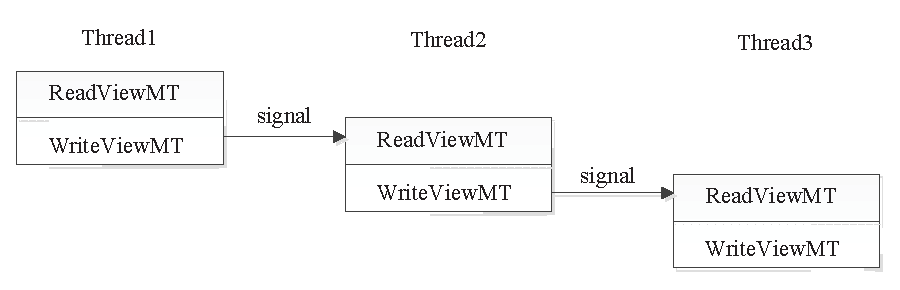
\includegraphics[width=3.1in]{../viewmt}
  \caption{Pipeline processing using ViewMTs. Access to a \code{ReadViewMT} is
  blocking until it is signaled. A stage sets its signal of \code{WriteViewMT}
after data processing is complete.}
  \label{fig:viewmt}
\end{figure}

%end of section.

\section{Implementation}
\label{sec:details}

We implement all the functionalities described before using C++
template metaprogramming technique. The grand idea is to utilize
template specialization and recursion to achieve control flow at
compile time. Besides template mechanism, other  C++ high level
abstracts act important roles in our approach. Function object and bind
mechnism is critical to postpone computation at proper place with
proper enviroment~\cite{moderncpp}. In order to utilize nested buiding blocks,
lambda expression can generate closure objects in a concise
form, e.g., line 24$\sim$37 of \reffig{sgemm}.

\subsection{Buiding Block Classes}

Implemenation of building blocks are straightforward. We use recursive calls
to support nesting patterns. \code{seq} and \code{par} are interoperable
because we chose proper nested class before calling function \code{apply}. Note that
building blocks do not know the nesting levels during the execution. To solve this
problem, each function object or cloure object is decorated with a loop-variable
counter.
%The handlers take responsibility for calculating loop variables in
%normalized form. It is only desirable for nested loop forms,
%\textit{e.g.} line 41 of List 1.
\todo{
Because some callable objects in C++ such as clousure object
do not provide default constructors, we pass their
references in those cases.  Consequently, some call sites of building blocks are different
from \reftable{bb}.}

For CPU, building blocks are implemented by embedding OpenMP directives. On GPU, we bind
building block classes to functions of OpenCL~\cite{opencl}, an open standard API
for heterogenous muliticores.

\subsection{TF class}

\code{TF\_hierarchy} has two template class definitions. The prime template
calls back task's inner function, while the partial specialization calls
leaf. We utilize predicate similar to Merge~\cite{merge} to generate subtasks
recursively. The main difference from Merge is that our predicate is a
\emph{metafunction} and is evaluated in place, e.g., line 3 below.

\begin{lstlisting}
  template <class TASK,
    template<class, class>  class PRED,
    bool SENTINEL = PRED<ARG0, ARG1>::value>
  struct TF_hierarchy{...}

  template <class TASK,
    template<class, class>  class PRED>
  struct TF_hierarchy<TASK, true>
  {...};
\end{lstlisting}

The \code{TF\_pipeline} class using variadic template~\cite{vartemp}. The
simplified implementation is listed as follows, which supports an arbitrary
number of functions. The only limitation is the maximal level of template
recursions of a compiler.

%For C++ compilers don't support variadic template, there
%are workarounds to achieve the same effect, but quite
%tedious.\footnote{zhangsq ask me to cite. I implemented the
 % workarounds myself, but i don't see it is necessary to show them here. too
 % details... --xliu 28. Nov}.

\begin{lstlisting}
 template <class P, typename... Tail>
  struct pipeline<P, Tail...> {
    typedef typename P::input_type in_t;
    typedef typename P::output_type out_t;
   
    static out_t doit(in_t in)
    {
     pipeline<Tail...>::doit( P::doit(in) );
    }
  };  
\end{lstlisting}

%end section

\section{Experiments and evalution}
\subsection{Methodology}\label{sectn:method}
%compiler and libs
We implement our library in standard
C++\cite{c++03, c++0x}. Theoretically, any standard-compliance C++ compiler
should process our classes without trouble. New C++ standard (a.k.a C++0x)\cite{c++0x} adds a
lot of language features to ease template metaprogramming. Compilers
without C++0x supports need some workarounds to pass compilation
though, they do not hurt expressiveness. Consider the trend of C++,
development of template library like libvina should become easier
and smoother in the future.  Currently, C++0x has been partially supported by some mainstreaming
compilers.  We developed the library and tested using GCC 4.4.0.  The
first implementation of OpenCL was shipped by Mac OSX 10.6. The GPU performance is collected on that platform.

A couple of algorithms are evaluated for our template approach.  They
are typical in image processing and scientific fields. In
addition, we implemented a psuedo language translation program to
illustrate pipeline processing. The programs in experiments are listed
as follows:

\begin{itemize}
\item[\textit{saxpy}] Procedure in BLAS level 1. A scalar multiplies to a single precision vector, which contains 32 million elements.
\item[\textit{sgemm}] Procedure in BLAS level 3. Two 4096*4096 dense matrices multiply.
\item[\textit{dotprod}] Two vectors perform dot production. Each vector
  comprises 32 million elements.
\item[\textit{conv2d}] 2-Dimensional convolution operation on image.  The Image
  is 4094*4096 black-white format. Pixel is normalized as a single
  float ranging from 0.0 to 1.0.
\item[\textit{langpipe}] Pseudo-Multi-language translation. A word is translated from one language A to language B, and then another function will translate it from language B to language C, etc.
\end{itemize}

Two multicore platforms are used to conduct experiments. The hardware
platforms are summed up in Table.~\ref{tbl:mach}

\begin{table}[hbt]
\caption{Experimental platforms}\label{tbl:mach}
\begin{center}
\begin{tabular}{|l|l|l|l|l|r|}
\hline
\textbf{name}&\textbf{type}&\textbf{processors}&\textbf{memory}&\textbf{OS}\\
\hline
harpertown&SMP &x86 quad-core  &4G&Linux Fedora\\
                  &  server &   
2-way  2.0Ghz & &kernel 2.6.30\\
\hline
macbookpro&laptop &x86 dual-core &2G&Mac OSX\\
                    &           & 2.63Ghz         &  &Snowleopard\\
                   &           &GPU 9400m    &256M & \\
                    &           & 1.1Ghz   & &\\
\hline
\end{tabular} 
\end{center}
\end{table}
On harpertown, we link Intel Math kernels to perform BLAS procedures
except for conv2d. On macbookpro, we implemented all the algorithms on
our own. For CPU platform, we link libSPMD thread library to
perform computation. The library binds CPUs for each SPMD
thread and switch to realtime scheduler on Linux.  This configuration
helps eliminate the impact of OS scheduler and other processes in the system.
\subsection{Evaluation}
\subsubsection{Speedup of Hierarchical transformation on CPU}
\begin{figure}
\includegraphics{speedupx86.0}
\caption{Speedup on Harpertown}\label{fig:spdx86}
\end{figure}

Fig.~\ref{fig:spdx86} shows the speedup on harpertown. The blade
server contains two quad-core Xeon
processors. We experiment SPMD transformation for algorithms. \textit{saxpy} and
\textit{conv2d} apply  \emph{TF\_mappar} while \textit{dotprod} and \textit{sgemm} apply \emph{TF\_mapreduce}.

We obverse good performance scalability for programs
\textit{conv2d} and \textit{sgemm}. \textit{conv2d} does not have any dependences
and it can obtain about 7.3 times speedup in our experiments. sgemm
needs an extra reduction for each division operation. The final
speedup is about 6.3 times when all the cores are available. It is worth noting that we
observe almost two-fold speedup from sequence to dual core. However,
the speedup degrates to 3.3 time when execution
environment change to 4-core. Harpertown consists of  2-way quad-core processors,  Linux
can not guarantee that 4 subprocedures are executed within a physical
processor. Therefore, the cost of memory accesses and synchronization
increases from 2-core to 4-core platform. 

\textit{dotprod} and \textit{saxpy} reveal low speedup because non-computation-intensive
programs are subject to memory bandwidth.  In average, \textit{saxpy} needs one load and one 
store for every two operations. \textit{dotprod} has similar
situation. They quickly saturate memory bandwidth for SMP system and
therefore perform badly. Even though we fully parallelize those
algorithms by our template library. 
\subsubsection{Speedup of  plain transformation on GPU}
\begin{figure}
\includegraphics{speedupgpu.0}
\caption{Speedup Comparing GPU with CPU}\label{fig:spdgpu}
\end{figure}

Fig.~\ref{fig:spdgpu} shows SPMD transformation results for GPU on
macbookpro. Programs run on host CPU  in sequence as
baseline. Embedded GPU on motherboard contains 2
SMs\footnote{Streaming Multiprocessor, each SM consists of 8 scalar processors(SP)}.
Porting from CPU to GPU, developer only need a couple of lines to change
templates while keeping algorithms same \footnote{
Because GPU code needs special qualifiers, we did modify kernel
functions a little manually.  Algorithms are kept except for sgemm. It is not easy
 to work out sgemm for a laptop, so we added blocking and SIMD
 instruments for CPU.}. As figure depicted,  computation-intensive programs
\textit{sgemm} and \textit{conv2d} still maintain their speedups. 4.5 to 5 times
performance boost is achieved for them by migrating to GPU.
In addition, we observe about 2 times performance boost for
\textit{saxpy}. Nvidia GPUs execute
threads in group of warp (32 threads) on hardware and it is
possible to coalesce memory accesses if warps satisfy
specific access patterns. Memory coalescence mitigates bandwidth issue
occurred on CPU counterpart. Because our program of \textit{dotprod} has fixed
step to access memory which does not fit any patterns, we can not
obtain hardware optimization without tweaking the algorithm.

\subsubsection{Comparison between different multicores}
\begin{table}[hbt]
\caption{Comparison of sgemm on CPU and GPU}\label{tbl:sgemm}
\begin{tabular}{|l|r|r|r|}
\hline
& baseline& CPU & GPU\\
\hline
\textbf{cores} &1 x86(penryn)& 8 x86(harpertown)& 2 SMs\\
\hline
\textbf{Gflops}& 2.64 &95.6&  12.0\\
\hline
\textbf{effectiveness}&12.6\%& 74.9\%&68.2\%\\
\hline
\textbf{lines of function}&63&unknown&21\\
\hline
\end{tabular}
\end{table}

Table.~\ref{tbl:sgemm} details \textit{sgemm} execution on CPU and GPU. Dense matrix
multiplication is one of  typical programs which have
intensive computation. Problems with this characteristic are the most
attractive candidates to apply our template-based approach.
Our template library transforms the \textit{sgemm} for both CPU and 
GPU. We choose sequential execution on macbookpro's CPU as
baseline. After mapping the algorithm to GPU, we directly obtains over
4.5 times speedup comparing with host CPU. Theoretically,  Intel Core
2 processor can issue 2 SSE instructions per cycle,  therefore, the
peak float performance is 21 Gflops on host CPU. We obtain 2.64 Gflops which
effectiveness is only 12.6\% even we employ quite complicated
implementation. On the other side, 12 Gflops is observed on GPU whose
maximal performance is roughly 17.6 Gflops.\footnote{$17.6Gflops = 1.1Ghz * 2(SM) *
  8(SP)$. nVidia declared their GPUs can perform a mad(multiply-add
  op) per cycle  for users who concern performance over precision. However, we can
  not observe mad hints bring any performance improvement in OpenCL. }
Although both column 2 and column 4 implement SIMD algorithm for
\textit{sgemm}, GPU's version is obviously easier and effective. It is
due to the dynamic SIMD and thread management from GPU
hardware~\cite{Fatahalian08} can significantly ease vector programming. Programmer can
implement algorithm in plain C and then replies on template
transformation for GPU.  Adapting \emph{TF\_mapreduce} template class
for GPU only need tens of lines code efforts. Like GPU template, we apply
\emph{TF\_mapreduce} to parallelize \textit{sgemm} procedure in MKL
for CPU. We observe 95.6 
Gflops and about 75\% effectiveness on harpertown server.

\subsubsection{Pipeline Transformation for CPU}
\begin{figure}[htp]
\includegraphics{pipeline.0}
\caption{Pipeline Processing for Psuedo Language Translation}\label{fig:pipe}
\end{figure}

Fig.~\ref{fig:pipe} demonstrates pipeline processing using our
template library. As described before, \textit{langpipe} simulates a
multilingual scenario. We apply template \emph{TF\_pipeline} listed in
Fig.~\ref{lst:pipe}. In our case, the program consists of  4 stages,
which can transitively translate English to Chinese\footnote{follow the 
  route: English  $\to$ French $\to$ Spanish $\to$ Italian $\to$
  Chinese}. Only the preceding stages complete,  it can proceed with
the next stages. The executing scenario is similar to Fig.~\ref{fig:viewmt}. We use bogus loop to consume $t \  \mu s$ on CPU. For each $t$, we iterate 500
times and then calculate the average consumptive time on harpertown. For
grained-granularity cases (20$\mu s$, 50$\mu s$, 100$\mu s$), we can obtain ideal
effectiveness in pipelining when 4 cores are exposed to the system.
\textit{i.e.} our program can roughly output one instance every $t\  \mu
s$. The speedup is easy to maintain when granularity is big. 100 $\mu s$ case ends up 54 $\mu s$ for each instance for 8 cores. 50  $\mu s$ case
bumps at 5 cores and then improves slowly along core increment. 20
$\mu s$ case also holds the trend of first two cases. 5 $\mu s$ case is
particular. We can not observe ideal pipelining until all 8
cores are available.  Our Linux kernel scheduler's granularity is 80
$\mu s$ in default. We think that the very fine granular tasks contend
CPU resources in out of the order. The runtime behavior presumably
incurs extra overhead. Many cores scenario helps alleviate the
situation and render regular pipeline processing.


\section{Related work}\label{sec:related}
%As mentioned before, it is desirable to extend conventional
%programming languages to reflects new hardwares. Researches in the field have two major directions:
To meet challenges of multicore, approaches based on existing
programming languages can be broadly categorized into two classes: A) library-based approaches, which
provide libraries to support parallel programs, and B) Compiler-based
approaches, which extend new language grammars or constructs for parallelism.

Library-based approaches extend programming languages
by well-developed libraries. Because both development and adaption of
the libraries are based on original language infrastructures, the
workload of programmers is relatively reduced. Many systems provide
such libraries to expose interfaces for parallel programs such as
Pthread (POSIX Thread), MPI (Message Passing Interface), and
OpenCL~\cite{opencl}. However, system-level libraries usually rely on 
their underlying platforms. Abstractions
of those libraries are usually far away from expressing parallelism
naturally, and it is difficult to
port programs from one library to another. Our library is a
metaprogramming library for source transformations. It contains template classes which abstract high-level parallel patterns
and executions, instead of the interfaces of system primitives or
resources. On the other side, system-level libraries, developing high-level
library to support parallelism and concurrency is also a hot topic in
programming language field~\cite{javacon, wincon}. C++ community intends to
achieve the target while bearing generic programming in mind.  TBB~\cite{tbb} has a plenty of
containers and building blocks to support loop-parallelism and
task-level parallelism.  Inspired by TBB's approach, we achieve the
same effects in static domain. We aim at using static information
to tailor to different multicore architectures. Besides, the template-based
approach we proposed is orthogonal to runtime parallel libraries. We
only exploit parallelism which can be resolved by compilers,
programmers feel free to employ other runtime approaches for further improvement.

%\textit{e.g.} Pthread is a
%\textit{de facto} standard interface of multithread for
%POSIX-compatible systems. 
%Furthermore, the implementation of thread on hardware is
%undefined in the standard, so it can not guarantee performance or even
%correctness on some architectures \cite{Boehm05}.

%Entities including partitioner and
%scheduler in TBB are created at run time. In that case, key data
%structures have to be thread-safe. Although TBB exploits task
%parallelism or other sophisticated concurrency on general purpose
%processors, the runtime overhead is relative high in data parallel
%programs, especially in the scenario that many lightweight threads are
%executing by hardware. 


%% MPI
%Another dominant parallel library is MPI in supercomputing community. It based on message-passing mechanism and SPMD model to execute parallel program. The difficulties of developing MPI programs are as notorious as pthread counterpart for programmers without sufficent training of parallel programming. 
%%

%OpenMP ~\cite{openmp} is designed for shared memory and has been shipped in almost every C/Fortran
%compilers.
%OpenMP can only perform Fork-Join parallel model.
%Source-to-Source transformation for optimization was reported by~\cite{Loveman77}, whose granularity of transformation  is
%statement.  Most of works have been merge in forms of IR in
%modern compilers. New source-to-source transformation compilers focus
%on function. 
%The run-time is usually provides in the form of dynamic link library.
%Although it is simple and
%portable, the performance is not optimal in most cases. Moreover, a
%handful of directives in OpenMP leave little room for further improving
%performance or scaling up to larger systems. Hybrid OpenMP with MPI is
%possible though, difficulties surge. 

In contrast, compiler-based approaches attempt to revise
programming languages per se. They add annotations or language constructs to
support parallel programs. Consequently, programmers
can describe parallel algorithms directly without caring about low-level executions.
OpenMP~\cite{openmp} compilers transform sequential code blocks into
multi-threaded equivalences according to directives. Although OpenMP
is \textit{de facto} standard for shared memory systems, it does not
support heterogeneous multicores. In order to achieve portability for
parallel programs, sequoia~\cite{sequoia, sequoia-compiler} transforms a \textit{task} into a cluster of
\emph{variants}, and uses Parallel Memory Hierarchy (PMH)
model~\cite{pmh} to map variants on physical architectures.
We derive the same idea from sequoia by transforming and mapping tasks
at compile time. Merge~\cite{merge} is a dynamic map/reduce programming
framework for heterogeneous multicores. It relies on the hierarchical division of tasks and predicate-based
dispatch system to assign tasks on matched targets at runtime. An obvious shortcoming of compiler-based approaches is that each
approach can only support one kind of parallel patterns. 

We intend to fuse the advantages of library-based approaches and
compiler-based approaches. Our approach performs source-to-source
transformations for different multicores by C++ template libraries. We
demonstrate that template metaprogramming is powerful enough to
implement multiple programming models.


%We think it is this process hardwires fixed parallel patterns into the
%compilers. Therefore, we explore the powerness of metaprogramming to
%transform sources for parallelism, which
%can support mulitple parallel programming models while maintain
%portability for multicores.

%First of all, it targets execution
%environment as a tree of machines, which an individual machine owns
%its storage and computation unit. Second, Target machine
%is described in XML files. \cite{sequoia} reports that Sequoia can transform programs
%for CellBE, cluster while keeping competitive performance. That
%is at expense of implementing one compiler for each platforms.
%The primary drawback of Sequoia is that its language constructs can not cover common
%parallel patterns such as pipeline or task queue. Methods mentioned before all need non-trivial efforts to
%modify compilers. As discussed in \cite{sequoia}, the authors of the Sequoia were
%still not clear whether the minimal set of primitives they provided provides can
%sufficiently express dynamic applications. We doubt if it is worthwhile to
%invest a compiler given the fact that template library can also
%achieve the same functionalities.

%end of section.
\section{Discussion and Future work}
The silicon industry has chosen multicore as new
direction. However, diverging multicore architectures enlarge the gap between algorithm-centric programmer and
computer system developers.  Conventional C/C++ programming language
can not reflect hardware essence any more.  Existing ad-hoc techniques
or platform-dependent programming language pose issues of generality
and portability. Source-to-source transformation can meet the challenge
and help tailor programs to specific multicore architectures.

%Not only the more processor cores but also
%elaborated memory hierarchy and exposed communication are adopted by
%new multicore architectures. More worse, 

We present a template metaprogramming approach to perform source-to-source
transformation for programs with rich information. Because it applies 
metaprogramming technique, template library is flexible enough to
apply any parallel
patterns and execution models. In addition, our approach
is extensible. Instead of modifying a compiler to add
annotations or language constructs, we implement the whole
functionalities by template mechanism. Template metaprogramming is
intimate for C++ programmers so they can extend the library to
facilitate proper parallel patterns and new architectural
features.  Our approach follows ISO C++ standards, which mean the
methodology is guaranteed to work across platforms.  Experiments shows
that our template approach can transform algorithms into SPMD threads
with competitive performance. These transformation are available for
both CPU and GPU, the cost of migration is manageable. We also
transform a group of standalone function wrappers into a
stream using our template library. It demonstrates that template
metaprogramming is powerful enough to support more than one parallel pattern.

%Our programming model bridges algorithm experts and diverging multcore
%architectures. Domain-specific experts focus on algorithms in form of
%conventional programming languages. They wrap functions to template
%classes and then pass them to \emph{TF class} as template parameter. Template
%mechniasm takes responisbility to transform source code according to
%their targets.

Streaming is an important computation model for innovative
multicore architectures. We partially exploit GPU functionality in this
paper though, transformation for GPU is quite
straightforward.  It is still unclear how many efforts need to
pay for a full-blown template library, which support
streaming computation. Libvina can only deal with regular
data. Future work on view class  will concentrate on supporting general operations like gather and scatter etc.  
Currently, kernel functions in GPU prohibit recursion. So we believe that
it is beneficial to introduce template recursion for GPU kernel functions. TF classes which support strip-mined memory access and loop iteration transformation are
particularly attractive for GPU targets because because  GPUs
provide memory coalescence for specific access patterns.

On CPU, source-to-source transformation should go on improving data
locality of programs. We plan to explore template approach to  generalize
blocking and tiling techniques.  It is also possible to re-structure
or prefetch data using template metaprograming accompanying with
runtime library.

General applications also contain a variety of static information to
optimize.The problem is that their memory footprints are irregular and
very hard to identify. It is desirable to explores new TF classes to facilitate
transforming source code close to target architectures using the static
information.

%\section*{Acknowledgements}

We would like to thank Weiliang Qian and Xiangyang Liu for helping me develop and test the codes.
We also thank Nicole Kwoh and Joanna Izabela Siebert for their technical discussions and proofreading.

This work is supported by the National High Technology Research and
Development Program (863 Program) of China (Grant No. 2006AA01Z172 and
2008AA01Z106), the National Natural Science Foundation of China (Grant
No. 60533040, 60725208 and 60773089), and Shanghai Pujiang Program
(Grant No. 07pj14049). This work is also partially supported by Hong Kong Polytehnic Univ under the grant
G-U513. 

\bibliographystyle{ieeetran}
\bibliography{../libvina}



% that's all folks
\end{document}
